\chapter[幻字]{幻字}
%\chapter[短标题显示在页面]{长标题显示在目录}

% {\small\textit{
% \quad Sors de l'enfance, ami réveille toi!\newline
% \quad \quad —Jean Jacques Rousseau.}
% \footnote{Ekster el infaneco,amiko veku!}
% \\}


\emoji{l_sena}

Soonoyun(你好)! 是我,Lein.今天我们来上第二课吧.
紫苑啊,你记住幻字的拉丁转写了吗?

\emoji{x_asex}

那是.我现在看转写词没啥问题,驾驶碰到"x"和"c"要小心. 
"x"发音像"shop"的"sh","c" 像西班牙语"burro"里的"rr".
把"c"当做[r]有点怪,但是我不想依赖别的例子去记它.
"シ"在Arka中写作"xi",所以我的名字在Arka里写作"Xion",不是"Shion".


\emoji{l_iks}

你别把xion读成ksion了,OK?

\emoji{x_seernik}

Xion... 我想到一个播放器\footnote{Zeon,瑞翁电器} :)

\emoji{l_niit}

先别管讲笑话,现在发音如何了?

\emoji{x_nal}
还是不习惯.但我会尽力去做的
让我试试这样行不行.顺便把字母表写下来.

% \includemedia[label=lettersong,flashvars={source=ARKA/hacm.mp3},
% transparent,
% passcontext %show VPlayer's right-click menu
% ]{}{APlayer.swf}\\
% \mediabutton[
% mediacommand=lettersong:play
% ]{\fbox{发音}}
% \mediabutton[
% mediacommand=lettersong:pause
% ]{\fbox{暂停}}

\begin{figure}[H]
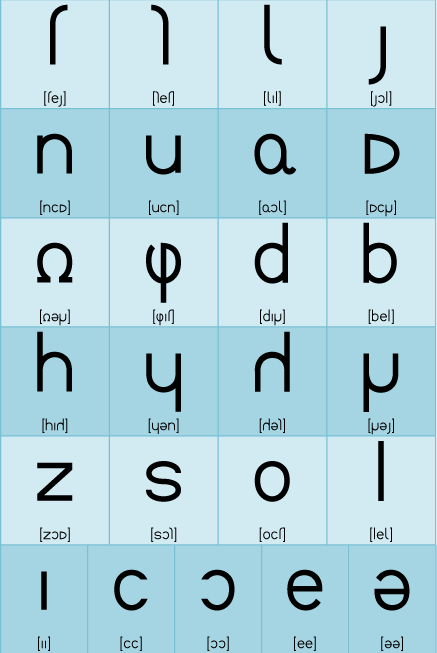
\includegraphics[width=0.5\textwidth]{ARKA/lemal.png}
\end{figure}
Yeah,这就挺不错的(=°ω°)ノニャン♪

"c"就像"burro"里的"rr",但是女生喜欢像日语的"r"一样发音就像"ramen"([ɾaːmen]). 
学术点的讲,就是齿龈闪音.

接下来,来听听\textattachfile{ARKA/hacm.mp3}
{字母歌}吧.
%"([a-z]+)"
%``$1''